\section{Domowa zupka typu instant}
\bigskip
\small
\begin{minipage}{0.45\textwidth}
    \noindent \textbf{Czas:} 10 minut \\
    \textbf{Poziom trudności:} łatwy
\end{minipage}
\begin{minipage}{0.45\textwidth}
    \noindent \textbf{Ilość sprzątania:} minimalna\\
    \textbf{Wymagany mysi sprzęt:} -
\end{minipage}
\normalsize
\vspace{0.5cm}

\begin{multicols}{2}

\subsection*{Składniki} \begin{itemize}
\item cienki makaron ryżowy (lub inny pszenny typu instant)
\item 2 łyżki sosu sojowego
\item 1 łyżeczka pasty miso (opcjonalnie, aczkolwiek zalecane)
\item 1/4 kostki bulionu warzywnego, drobiowego lub wołowego
\item 1/2 łyżeczki oleju sezamowego
\item wybrane źródło białka (np. kostki tofu lub kawałki tzw. "kurczaka z rożna")
\item różne warzywa wedle uznania, świeże lub mrożone (np. floretki brokułu, cienkie paski marchewki, zielona cebulka, groszek zielony, itp.)
\end{itemize}

\columnbreak

\begin{figure}[H]
    \centering
    \fbox{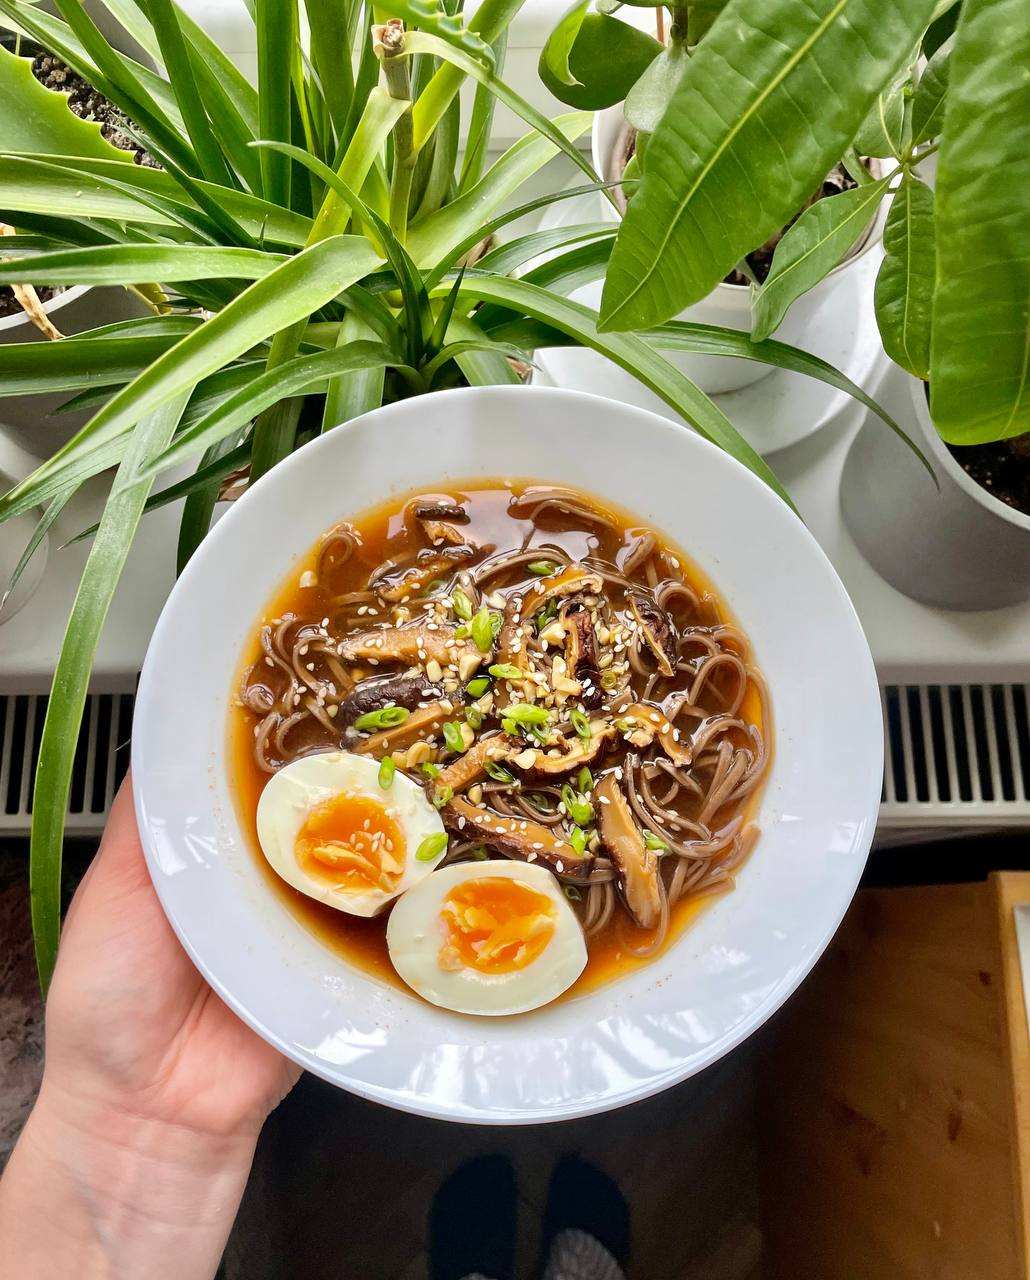
\includegraphics[width=0.35\textwidth]{images/zupka-instant.jpg}}
\end{figure}
\end{multicols}

\vspace{0.5cm}

\subsection*{Instruktaż}
\begin{enumerate}
    \item Na dnie średniej wielkości miski wymieszać ze sobą dokładnie sos sojowy, olej sezamowy, pastę i bulion.
    \item Warzywa pokroić na kawałki takiej wielkości, aby mogły ugotować się w kilka minut, tzn. marchewkę w drobną kostkę lub cienkie paski, brokuła rozdrobnić na małe floretki, itp.
    \item Pokrojone warzywa, tofu/kurczaka oraz makaron przełożyć do miski z sosem i zalać odpowiednią ilością wrzątku. Trzymać całość pod przykryciem przez ok. 5 minut lub do otrzymania pożądanej konsystencji makaronu. W razie potrzeby przyprawić do smaku sosem sojowym.
\end{enumerate}

\vspace{0.5cm}

\small \subsection*{Propozycja podania} Z jajkiem ugotowanym na miękko, z ziarenkami sezamu, z zieloną cebulką, z grzybami shiitake.

\vspace{0.3cm}

\subsection*{Dodatkowe uwagi} Danie można bardzo łatwo dostosować do wzięcia w drogę — wszystkie składniki wystarczy uprzednio włożyć do zamykanego pudełka na żywność wielokrotnego użytku lub szklanego słoika i zalać wrzątkiem w odpowiedniej chwili.

\newpage
